\documentclass{standalone}

% Plotting
\usepackage{tikz}
\usetikzlibrary{decorations.markings}
\usetikzlibrary{calc}
% quantikz breaks tikz-cd, see https://tex.stackexchange.com/questions/618330/quantikz-breaks-spacing-in-tikz-matrices-tikz-cd
%\usetikzlibrary{quantikz}
\usetikzlibrary{cd}
\usepackage{pgfplots}

\usepackage{simpler-wick}
\usepackage{physics}

\usepackage{amsmath}
\usepackage{mathtools}

\begin{document}
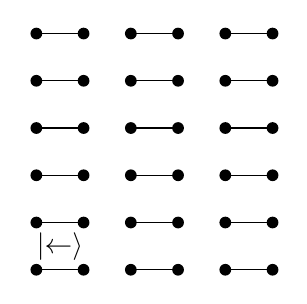
\begin{tikzpicture}[scale=1.5, decoration={
    markings,
    mark=at position 0.5 with {\arrow{>}}}]

    \foreach \i in {0,0.4,...,2} {
        \foreach \j in {0,0.4,...,2} {
            \node at (\i, \j) [circle,fill,inner sep=1.5pt]{};
        }
    }
    \foreach \i in {0,0.8,...,1.6} {
        \foreach \j in {0,0.4,...,2} {
            \draw (\i, \j) --++ (0.4, 0);
        }
    }
    \draw (0.2, 0) node[above] {$\ket{\leftarrow}$};
\end{tikzpicture}
\end{document}